\documentclass[a4paper, 12pt]{article}

%%% SST LAB PROTOCOLL PREAMBLE
%%% 2019
%%%%%%%%%%%%%%%%%%%%%%%%%%%%%%%


%%% PACKAGES
%%%%%%%%%%%%%%%%%%%%%%%%%%%

\usepackage[ngerman]{babel}

\usepackage[utf8]{inputenc}
\usepackage{amsmath}
\usepackage{pgfplots}
\usepackage{tikz}
\usepackage[many]{tcolorbox}
\usepackage{graphicx}
\graphicspath{ {./graphics/} }
\usepackage{pdfpages}
\usepackage{dashrule}
\usepackage{float}
\usepackage{siunitx}
\usepackage{trfsigns}
\usepackage{booktabs}
\usepackage[european]{circuitikz}
\usepackage{tcolorbox}

%%% DOCUMENT GEOMETRY
%%%%%%%%%%%%%%%%%%%%%%%%%%%

\usepackage{geometry}
\geometry{
 a4paper,
 total={0.6180339887498948\paperwidth,0.6180339887498948\paperheight},
 top = 0.1458980337503154\paperheight,
 bottom = 0.1458980337503154\paperheight
 }
\setlength{\jot}{0.013155617496424828\paperheight}
\linespread{1.1458980337503154}

\setlength{\parskip}{0.013155617496424828\paperheight} % paragraph spacing


%%% COLORS
%%%%%%%%%%%%%%%%%%%%%%%%%%%

\definecolor{red1}{HTML}{f38181}
\definecolor{yellow1}{HTML}{fce38a}
\definecolor{green1}{HTML}{95e1d3}
\definecolor{blue1}{HTML}{66bfbf}
\definecolor{hsblue}{HTML}{00b1db}
\definecolor{hsgrey}{HTML}{afafaf}

%%% CONSTANTS
%%%%%%%%%%%%%%%%%%%%%%%%%%%
\newlength{\smallvert}
\setlength{\smallvert}{0.0131556\paperheight}


%%% COMMANDS
%%%%%%%%%%%%%%%%%%%%%%%%%%%

% differential d
\newcommand*\dif{\mathop{}\!\mathrm{d}}

% horizontal line
\newcommand{\holine}[1]{
  	\begin{center}
	  	\noindent{\color{hsgrey}\hdashrule[0ex]{#1}{1pt}{3mm}}\\%[0.0131556\paperheight]
  	\end{center}
}

% mini section
\newcommand{\minisec}[1]{ \noindent\underline{\textit {#1} } \\}

% quick function plot
\newcommand{\plotfun}[3]{
  \vspace{0.021286\paperheight}
  \begin{center}
    \begin{tikzpicture}
      \begin{axis}[
        axis x line=center,
        axis y line=center,
        ]
        \addplot[draw=red1][domain=#2:#3]{#1};
      \end{axis}
    \end{tikzpicture}
  \end{center}
}

% box for notes
\newcommand{\notebox}[1]{

\tcbset{colback=white,colframe=green1!100!black,title=Note!,width=0.618\paperwidth,arc=0pt}

 \begin{center}
  \begin{tcolorbox}[]
   #1 
  \end{tcolorbox}
 
 \end{center} 
 
}

% box for equation
\newcommand{\eqbox}[2]{
	
	\tcbset{colback=white,colframe=green1!100!black,title=,width=#2,arc=0pt}
	
	\begin{center}
		\begin{tcolorbox}[ams align*]
				#1
		\end{tcolorbox}
		
	\end{center} 
	
}
% END OF PREAMBLE

%%%%%%%%%%%%%%%%%%%%%%%%%%%%%%%%%%%%%

\begin{document}

%%%%%%%%%%%%%%%%%%%%%%%%%%%%%%%%%%%%%
  
\includepdf{./titlepage/titlepage.pdf}
  \clearpage
  \setcounter{page}{1}
%%%%%%%%%%%%%%%%%%%%%%%%%%%%%%%%%%%%%

\section{Versuchsdurchführung}

Als Basismaterial der Bedampfung wurde ein Kunststoffplättchen verwendet, auf welches Kupfer aufgedampft werden sollte.

\subsection{Reinigung des Substrats}
Im ersten Versuchsschritt erfolgte die Reinigung des Substrats in
insgesamt drei Durchläufen im $60\si{\celsius}$ warmen Ultraschallbad, je 3
Minuten. Die erste Reinigung wurde mit Trichlorethen (Entfettung), die
zweite mit Aceton und die dritte mit Methanol (Entfernung der Stoffreste der
vorherigen Reinigungen) durchgeführt. Anschließend wurde das Substrat mit
Löschpapier getrocknet und danach gewogen.

\subsection{Wägung des Substrats}
Ziel war es, die Masse des unbedampften und des bedampften Substrats zu messen und durch Differenzbildung die Aufgedampfte Kupfermasse zu ermitteln. Die Ausgangsmasse des Substrats wurde
mit einer ``Kern 870'' Waage mit einer Anzeigegenauigkeit von $0.1 \,  \si{\milli\gram}$
und einer Messabweichung von XXXX gemessen.
\begin{table}[H]
  \begin{center}
    \begin{tabular}{@{}ll@{}}
      \toprule
      $n$ & $m_n \, / \si{\gram}$ \\ \midrule
      1  & 1.9628 \\
      2  & 1.9628 \\
      3  & 1.9630 \\
      4  & 1.9627 \\
      5  & 1.9629 \\
      6  & 1.9629 \\
      7  & 1.9629 \\
      8  & 1.9628 \\
      9  & 1.9628 \\
      10 & 1.9629 \\ \bottomrule
    \end{tabular}
  \end{center}
  \caption{Messreihe der Substratmasse vor der Bedampfung}
\end{table}

\noindent Der Mittelwert der Messreihe ergibt sich zu:
$$\bar{g} = 1.9630 \, \si{\gram}$$

\noindent Die Standardabweichung konnte mit

$$\sigma = \sqrt{ \frac{1}{N-1} \sum_{n=1}^{N}{( g_n - \bar{g} ) ^2} }$$

\noindent ermittelt werden. Sie beträgt\\
$$\sigma = 1.79505 \cdot 10^{-4} \, \si{\gram}$$

\noindent Mit einem Vertrauensbereich von $1 \cdot \sigma$ ergibt sich die Ausgangsmasse
$$m_1 = 1.9630 \, \si{\gram} \pm 0.00914 \, \si{\percent}$$

\subsection{Bedampfung des Substrats}
Vor dem Bedampfen wurde das Substrat auf eine Maskenform mit einer Fläche von ca. $1.16
\,\si{\centi\meter} \cdot 2.83\, \si{\centi\meter}$ befestigt.

Die Bedampfung wurde mittels Physical-Vapour-Deposition-Verfahren (PVD) durchgeführt. Das Kupfer wurde auf das sogenannte "boat" (Schiff) innerhalb der Vakuumkammer gelegt, wo es nach Evakuierung bei einem Druck von $XXXX \, \si{\milli\bar}$ durch elektrischen Strom erwärmt und geschmolzen wurde. Vor dem Schmelzvorgang wurden die Oberflächen innerhalb der Kammer mithilfe von ionisierten Gasen bei hoher Spannung ($500 \, \si{\volt}$) gereinigt (Plasmareinigung, Abbildung 2).\\

\begin{figure}[H]
	\begin{center}
		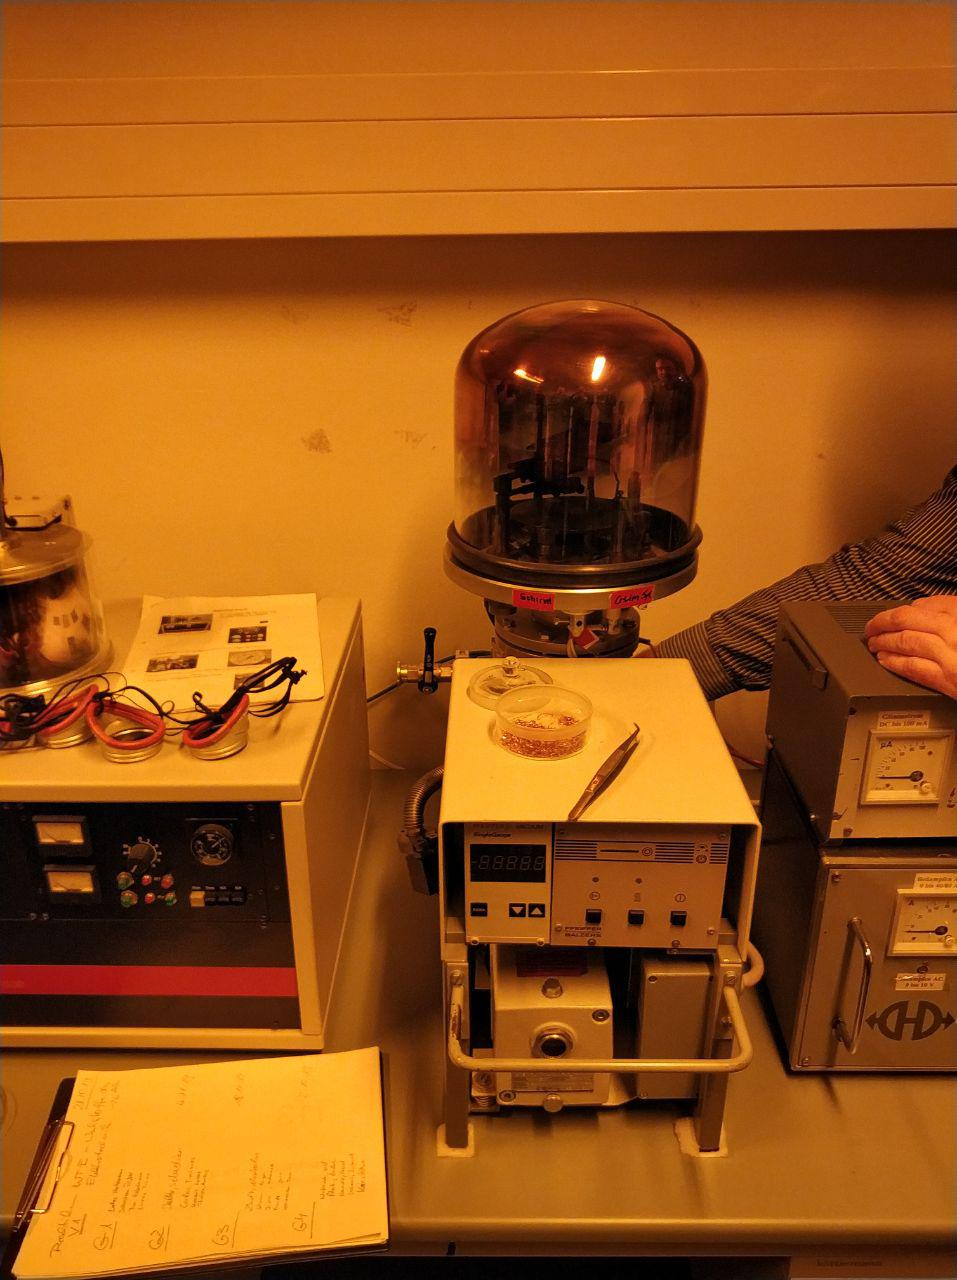
\includegraphics[width=\textwidth]{aufbau}
	\end{center}
	\caption{Versuchsaufbau}
\end{figure}

\begin{figure}[H]
	\begin{center}
		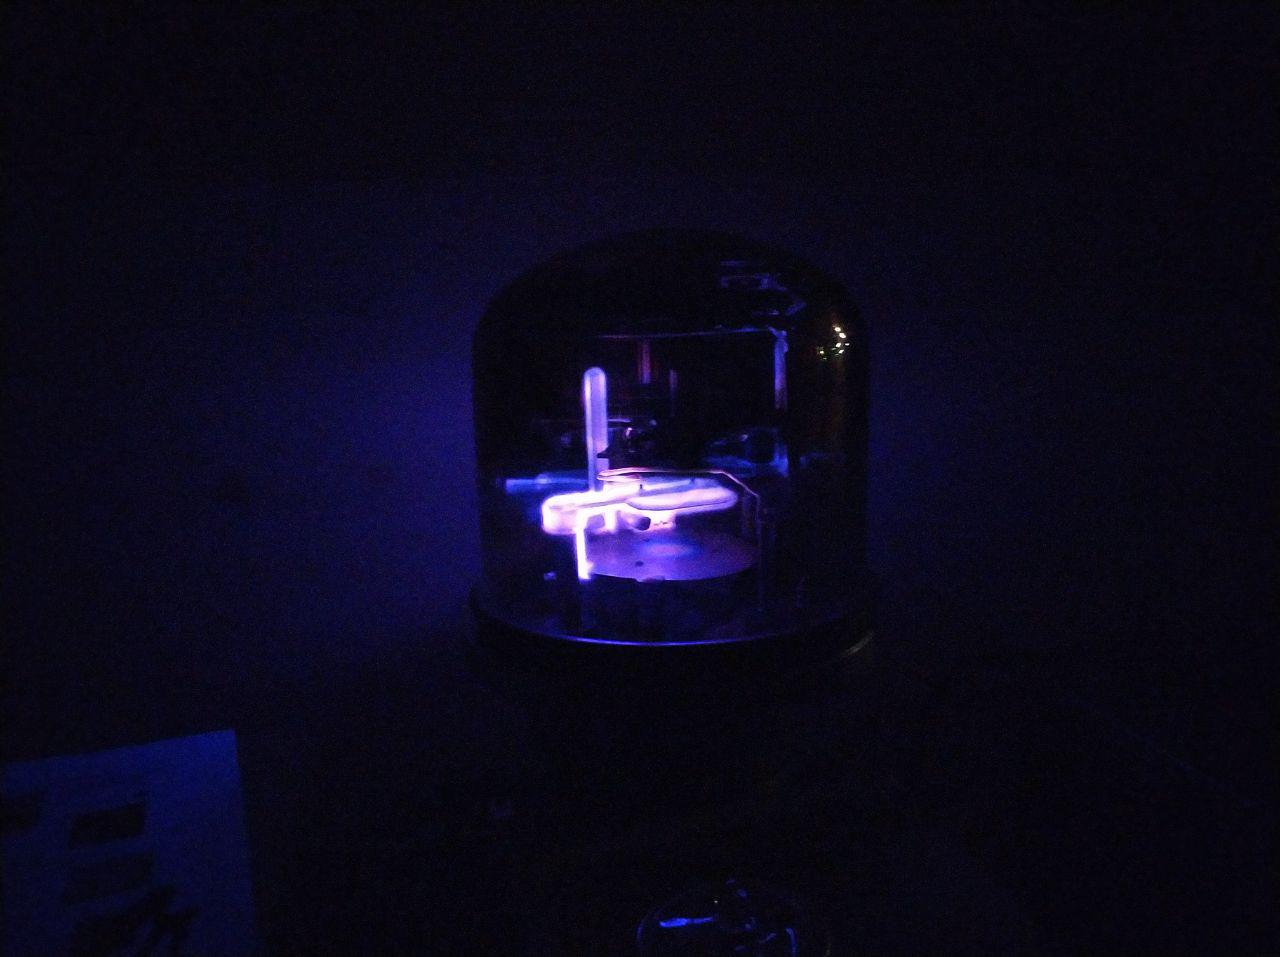
\includegraphics[width=\textwidth]{plasma}
	\end{center}
	\caption{Plasmareinigung}
\end{figure}

\begin{figure}[H]
\begin{center}
	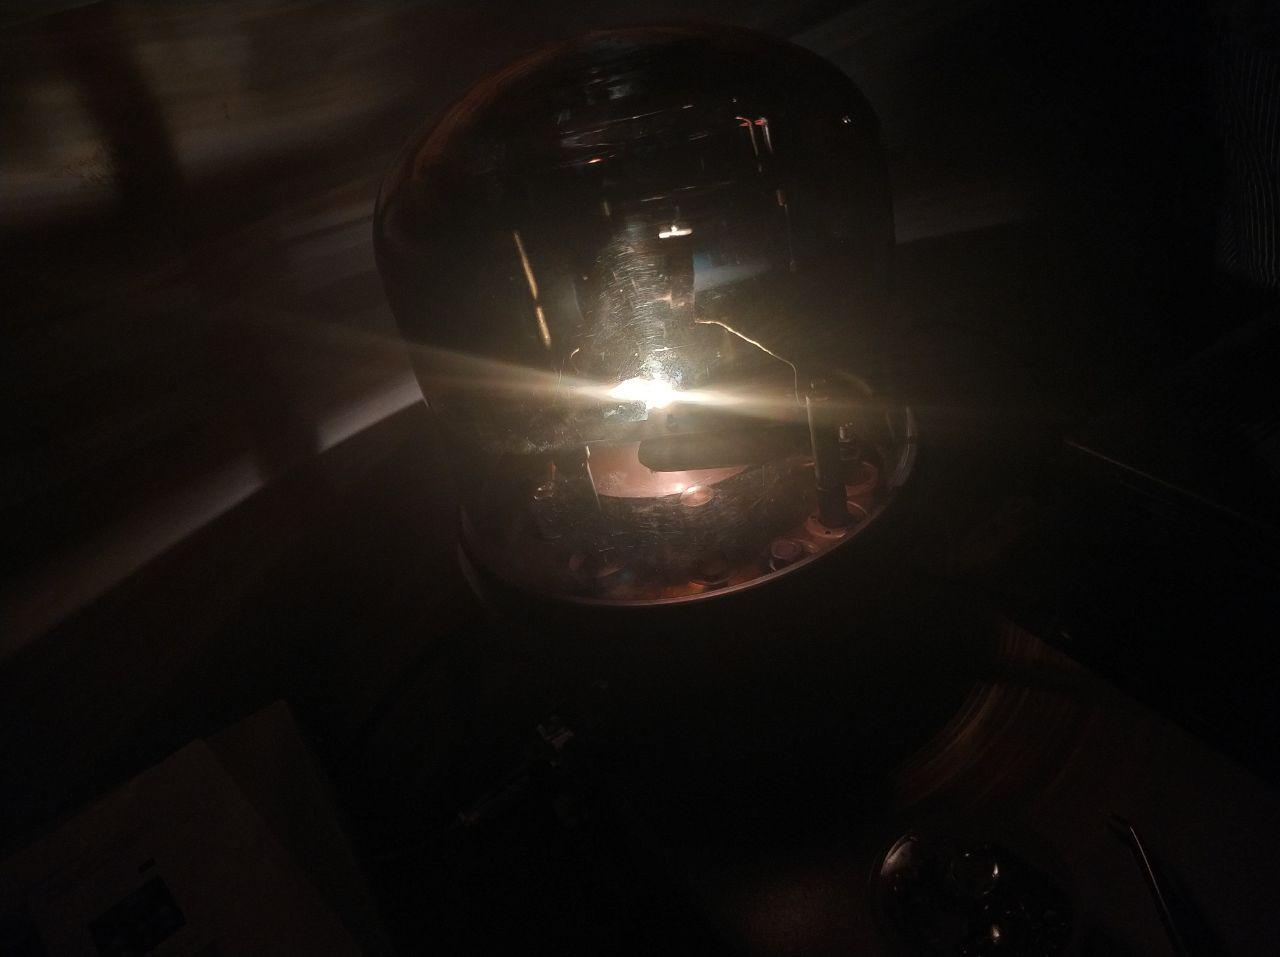
\includegraphics[height=0.618\textwidth]{weiss}
\end{center}
\caption{Weißes Glühen des Kupfers}
\end{figure}


\begin{figure}[H]
	\begin{center}
		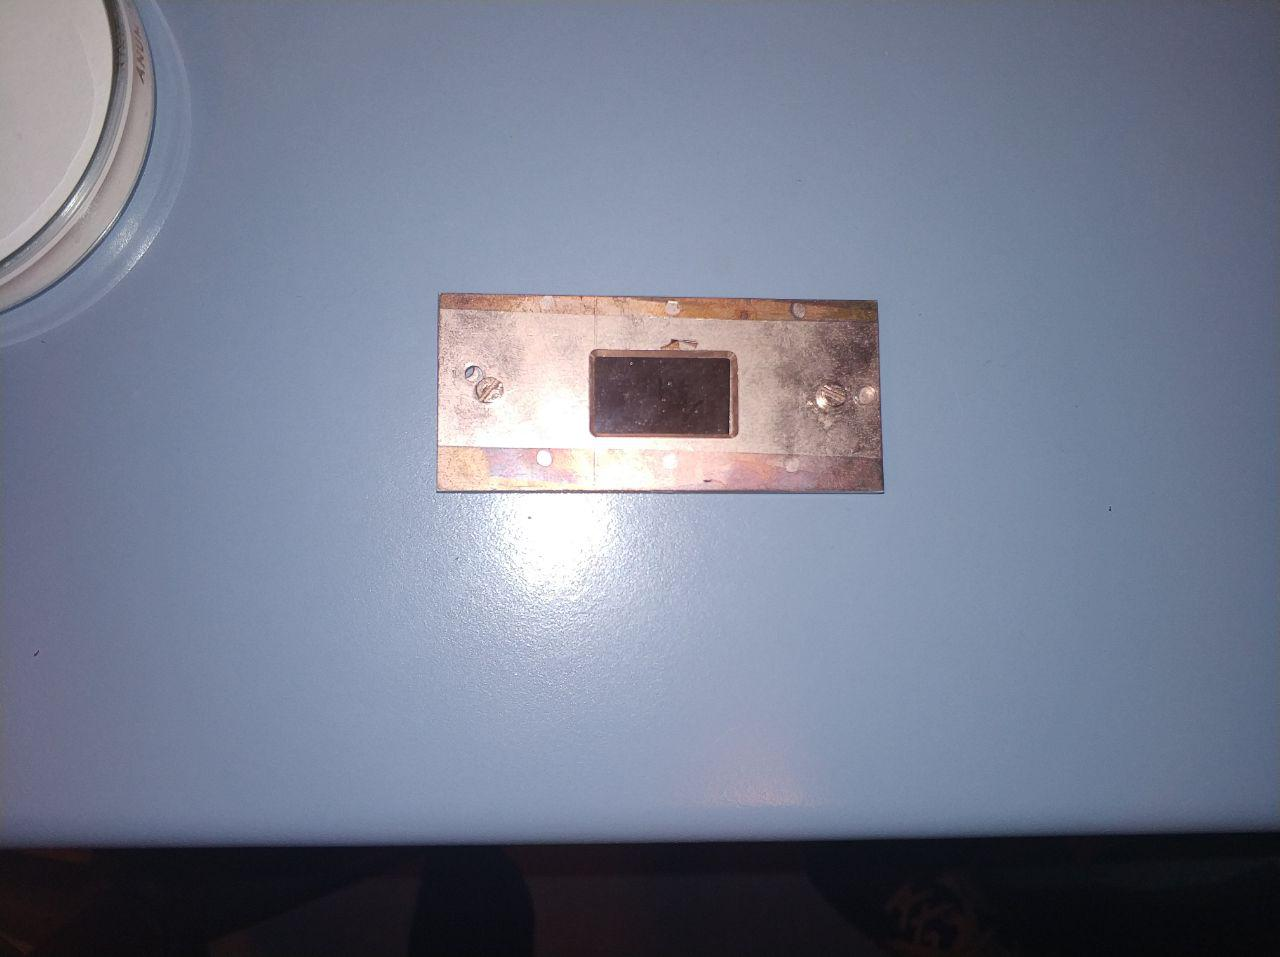
\includegraphics[height=0.618\textwidth]{befestigt}
	\end{center}
\caption{Bedampftes Substrat in der Maskenform}
\end{figure}

\section{Ergebnis}
Der erste Versuch der Bedampfung ist leider fehlgeschlagen, da die Blende über dem boat nach der Plasmareinigung nicht zurückgestellt wurde und somit die Blende und nicht das Substrat bedampft wurde. 

Der zweite Versuch gelang vorerst. Während der Bestimmung der bedampften Fläche unter dem Lichtmikroskop hat sich jedoch das Kupfer vom Substrat gelöst (Abbildung X), wodurch die Messung der Massendifferenz nicht mehr möglich war.

\noindent Mögliche Gründe für das Ablösen der Kupferschicht sind:
\begin{itemize}
	\item Zu hohe Kupfermasse \\$\rightarrow$ Bedampfte Schichtdicke zu hoch\\ $\rightarrow$ stärkere innere Spannungen des Kupfers aufgrund der unterschiedlichen Wärmeausdehnungskoeffizienten von Kupfer und Substrat.
	\item yes
\end{itemize}  

\begin{figure}[H]
	\begin{center}
		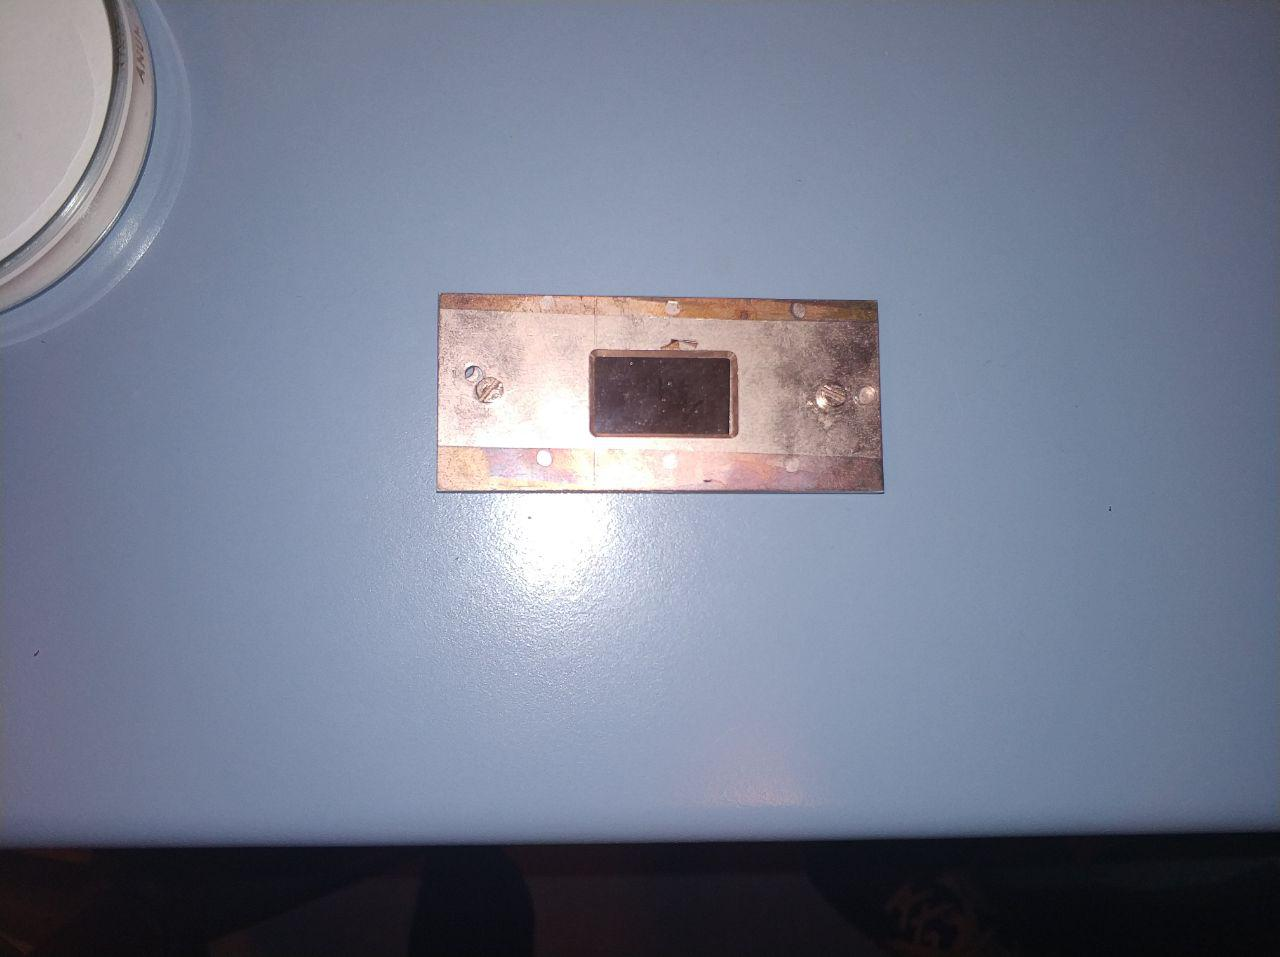
\includegraphics[width=\textwidth]{befestigt}
	\end{center}
	\caption{Bedampftes Substrat in der Maskenform}
\end{figure}

\begin{figure}[H]
	\begin{center}
		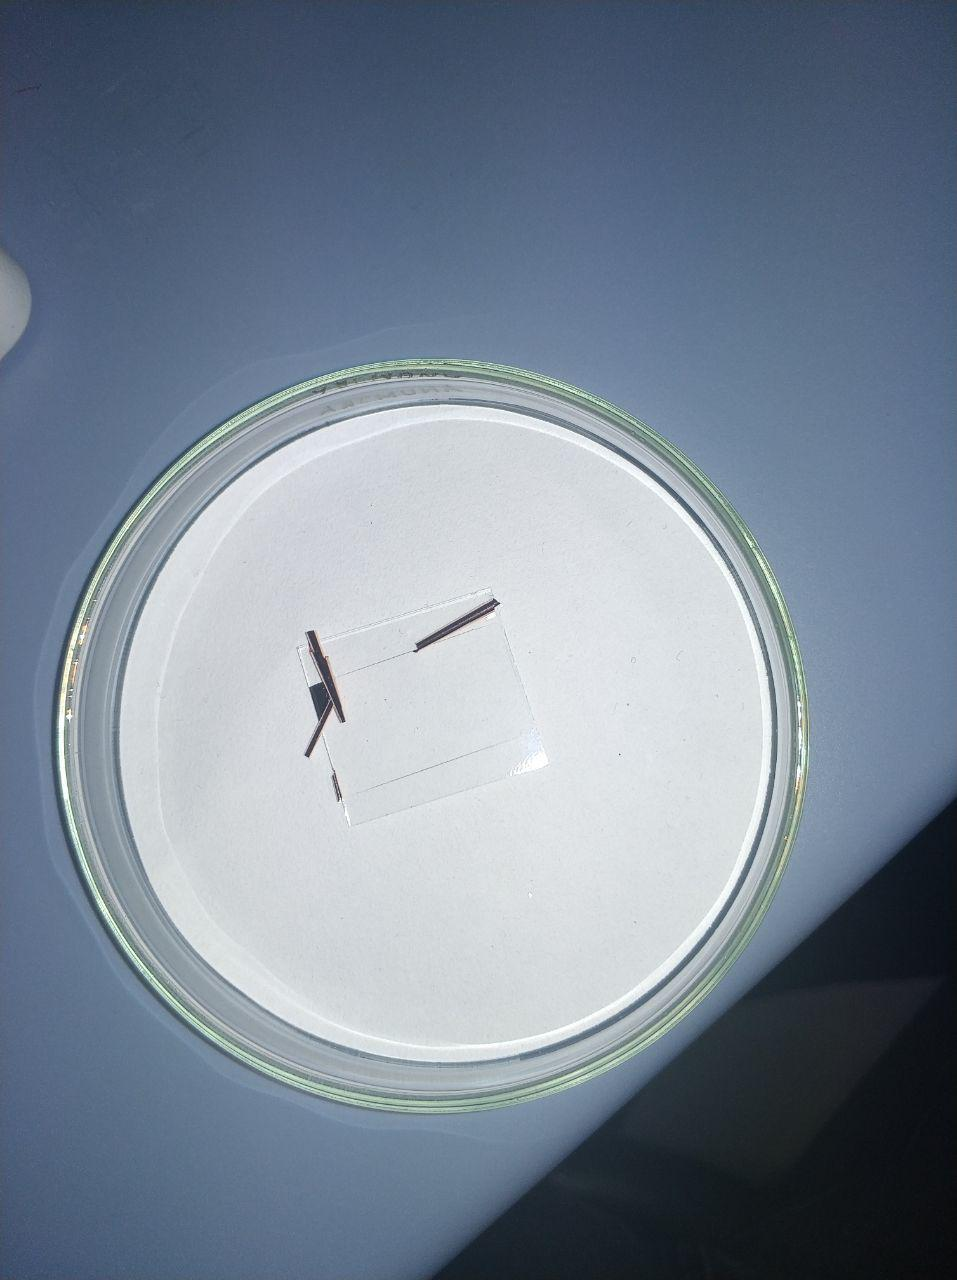
\includegraphics[width=\textwidth]{kaputt}
	\end{center}
	\caption{Ergebnis des zweiten Bedampfungsversuchs}
\end{figure}


\end{document}
